\section{Résultats}

\paragraph{Mesure de la viscosité} La viscosité \(\eta\) de chaque huile à différentes températures a été déterminée à partir de l'\autoref{eq:viscosite}. La température de chaque huile a été variée entre \mbox{\(T=(22 \pm 1)\) \si{\celsius}} et \mbox{\(T=(72 \pm 1)\) \si{\celsius}} pour la température ascendante, notée \(T\nearrow\), et entre \mbox{\(T=(72 \pm 1)\) \si{\celsius}} et \mbox{\(T=(29 \pm 1)\) \si{\celsius}} pour la température descendante, notée \(T\searrow\). Les densités utilisées pour les huiles 1 et 2 sont respectivement \(\rho_1 = 819\) \si{\kilo\gram\per\cubic\meter} et \(\rho_2 = 837\) \si{\kilo\gram\per\cubic\meter} \cite{val_ref}. Les détails sur le calcul d'erreurs sont disponibles en \autoref{sec:erreurs}. Les résultats obtenus sont reportés dans les \autoref{fig:huile1_eta} et \autoref{fig:huile2_eta}. Afin d'alléger les figures dans tout le rapport, seul une partie des mesures sont montrées.

\begin{figure}[h]
    \centering
    \begin{subfigure}{0.48\linewidth}
        \centering
        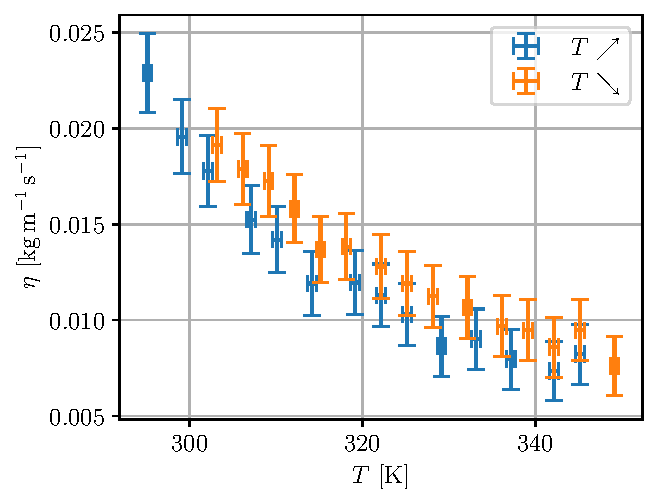
\includegraphics[width=\linewidth]{figures/huile1_eta.pdf}
        \caption{}
        \label{fig:huile1_eta}
    \end{subfigure}
    \begin{subfigure}{0.48\linewidth}
        \centering
        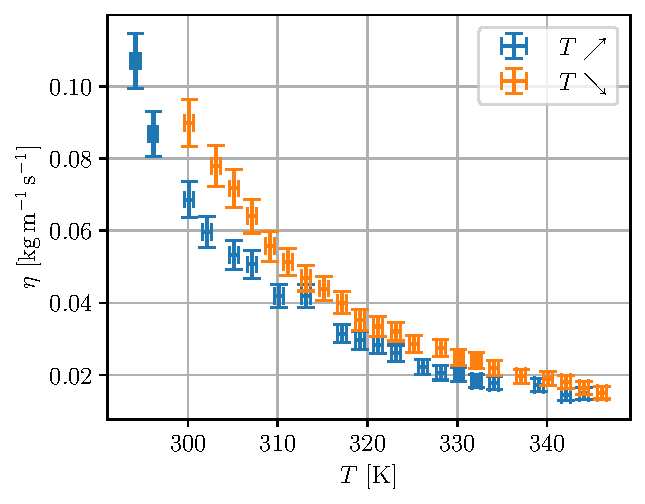
\includegraphics[width=\linewidth]{figures/huile2_eta.pdf}
        \caption{}
        \label{fig:huile2_eta}
    \end{subfigure}
    \caption{Viscosité \(\eta\) en fonction de la température dans le sens croissant ou décroissant dans l'huile (a) 1, (b) 2}
\end{figure}

Afin d'obtenir l'énergie d'activation \(E\), ainsi qu'une constante \(A\), une régression linéaire est réalisée sur les \autoref{fig:huile1_lneta} et \autoref{fig:huile2_lneta}, conformément à l'\autoref{eq:ln_relation_boltzmann}. Les valeurs obtenues sont reportées dans le \autoref{tab:energie_fit}.

\begin{figure}[h]
    \centering
    \begin{subfigure}{0.48\linewidth}
        \centering
        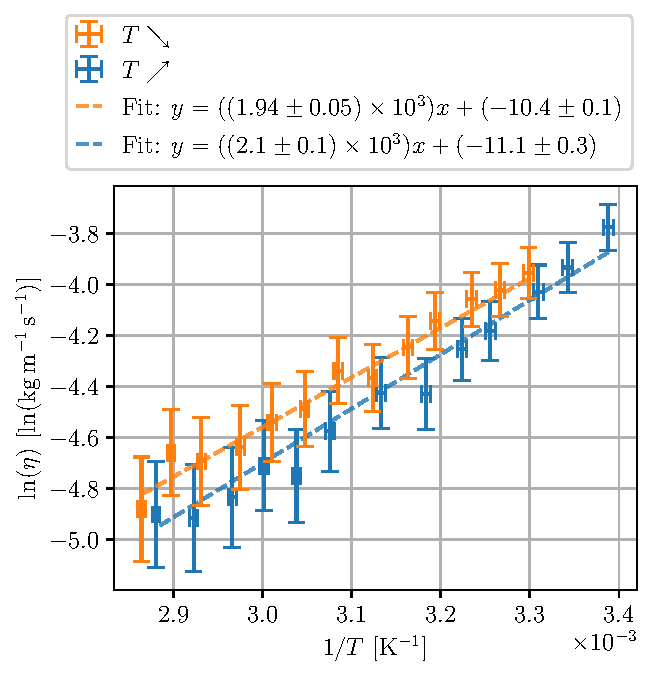
\includegraphics[width=\linewidth]{figures/huile1_lneta.pdf}
        \caption{}
        \label{fig:huile1_lneta}
    \end{subfigure}
    \begin{subfigure}{0.48\linewidth}
        \centering
        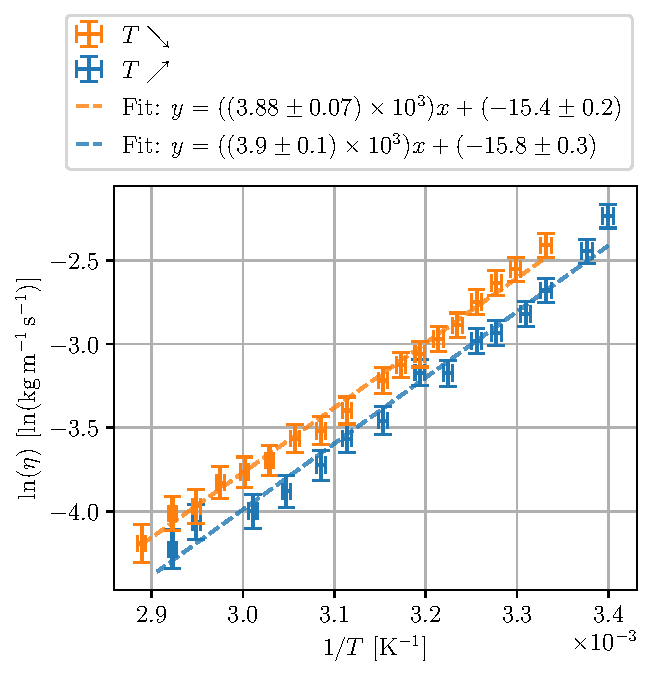
\includegraphics[width=\linewidth]{figures/huile2_lneta.pdf}
        \caption{}
        \label{fig:huile2_lneta}
    \end{subfigure}
    \caption{Logarithme de la viscosité \(\ln(\eta)\) en fonction de l'inverse de la température \(T\) dans (a) l'huile 1 et (b) l'huile 2}
\end{figure}

\begin{table}[h]
    \centering
    \begin{tabulary}{0.8\linewidth}{C C|C C}
        \toprule
        & & \(E\) [\si{\joule}] & \(A\) [\si{\kilo\gram\per\meter\per\second}] \\
        \midrule
        Huile 1 & \(T \nearrow\) & \((2.9 \pm 0.2) \cdot 10^{-20}\) & \((1.5 \pm 0.5) \cdot 10^{-5}\) \\
        & \(T \searrow\) & \((2.68 \pm 0.06) \cdot 10^{-20}\) & \((3.1 \pm 0.4) \cdot 10^{-5}\) \\
        \midrule
        Huile 2 & \(T \nearrow\) & \((5.4 \pm 0.1) \cdot 10^{-20}\) & \((1.3 \pm 0.4) \cdot 10^{-7}\) \\
        & \(T \searrow\) & \((5.35 \pm 0.09) \cdot 10^{-20}\) & \((2.0 \pm 0.4) \cdot 10^{-7}\) \\
        \bottomrule
    \end{tabulary}
    \caption{Valeurs de l'énergie d'activation \(E\) et la constante \(A\) pour des mesures à température croissante et décroissante des huiles 1 et 2}
    \label{tab:energie_fit}
\end{table}

La viscosité cinématique autour de \(T = 40\) \si{\celsius} est obtenue avec \(\nu = \frac{\eta}{\rho}\). Ces valeurs sont alors comparées avec les valeurs données par le fabricant dans le \autoref{tab:val_ref}.

\begin{table}[h]
    \centering
    \begin{tabulary}{0.8\linewidth}{C C|C|C C}
        \toprule
        & & \(\nu_\textrm{ref}\) [\si{\square\milli\meter\per\second}] & \(\nu_{T=40 \si{\celsius}}\) [\si{\square\milli\meter\per\second}] & Écart relatif [\%] \\
        \midrule
        Huile 1 & \(T \nearrow\) & 15 & \(15 \pm 2\) & \(5\) \\
        & \(T \searrow\) &  & \(19 \pm 2\) & \(30\) \\
        \midrule
        Huile 2 & \(T \nearrow\) & 68 & \(50 \pm 4\) & \(26\)\\
        & \(T \searrow\) &  & \(56 \pm 4\) & \(18\) \\
        \bottomrule
    \end{tabulary}
    \caption{Viscosité cinématique autour de \(T = 40\) \si{\celsius} comparé aux valeurs de référence \cite{val_ref} pour des mesures à température croissante et décroissante des huiles 1 et 2}
    \label{tab:val_ref}
\end{table}

\paragraph{Calcul du nombre de Reynolds}
La formule de Stokes utilisée pour obtenir l'\autoref{eq:trainee_stokes} a un intervalle de validité de $0 \leq \mathrm{Re} \leq 0.5$. Le nombre de Reynold a donc été calculé pour chaque mesure effectuée à l'aide de l'\autoref{eq:Reynolds} et des valeurs de $\eta$ calculées précedemment. Les résultats sont reporté dans les \autoref{fig:huile1_Re} et \autoref{fig:huile2_Re}. Il est possible d'observer que pour l'huile 1 l'intervalle n'est pas respecté ou alors simplement pour les toutes premières mesures. Pour l'huile 2 l'intervalle est respecté jusqu'à la température de 320 \si{\kelvin} après quoi le nombre de Reynold dépasse largement les limitations.
\begin{figure}[H]
    \centering
    \begin{subfigure}{0.48\linewidth}
        \centering
        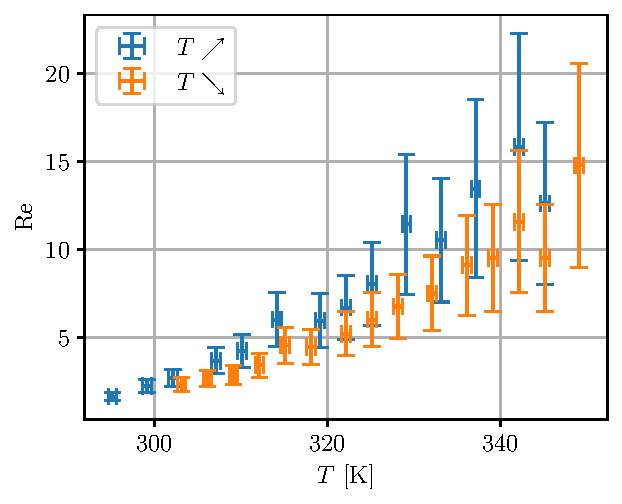
\includegraphics[width=\linewidth]{figures/huile1_Re.pdf}
        \caption{}
        \label{fig:huile1_Re}
    \end{subfigure}
    \begin{subfigure}{0.48\linewidth}
        \centering
        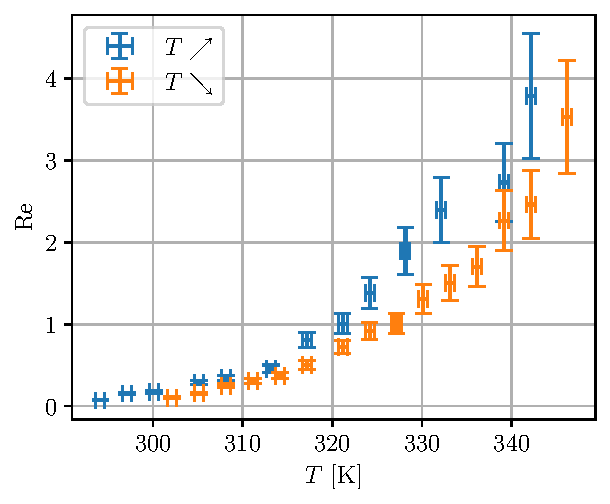
\includegraphics[width=\linewidth]{figures/huile2_Re.pdf}
        \caption{}
        \label{fig:huile2_Re}
    \end{subfigure}
    \caption{Nombre de Reynolds en fonction de la température pour la bille chutant à sa vitesse maximale pour (a) l'huile 1 et (b) l'huile 2}
\end{figure}

\paragraph{Constante de temps} A l'aide de l'\autoref{eq:constante_temps} et des études précédentes il a été possible de déterminer la valeur de la constante de temps pour la convergence de la vitesse vers la vitesse d'équilibre. L'information importante a retirer de cette analyse étant le nombre de constante de temps qui se sont écoulés les valeurs de $t_1/\tau$ pour chaque mesure ont été calculées, avec $t_1$ le temps auquel la mesure de la vitesse commence. Les résultats sont reportés dans les \autoref{fig:huile1_tau} et \autoref{fig:huile2_tau}.
\begin{figure}[H]
    \centering
    \begin{subfigure}{0.48\linewidth}
        \centering
        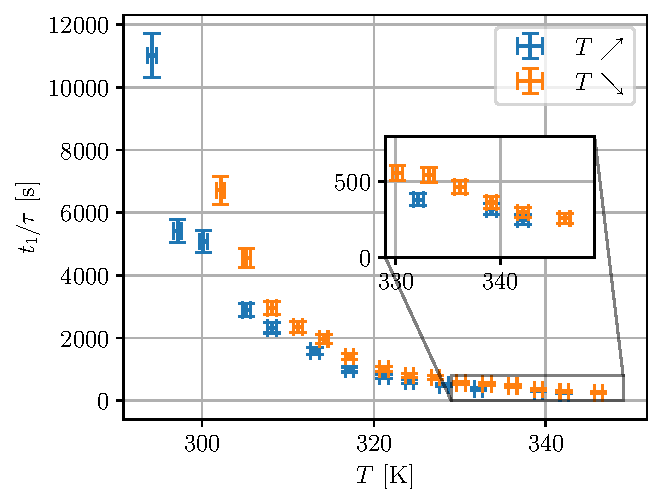
\includegraphics[width=\linewidth]{figures/huile1_tau.pdf}
        \caption{}
        \label{fig:huile1_tau}
    \end{subfigure}
    \begin{subfigure}{0.48\linewidth}
        \centering
        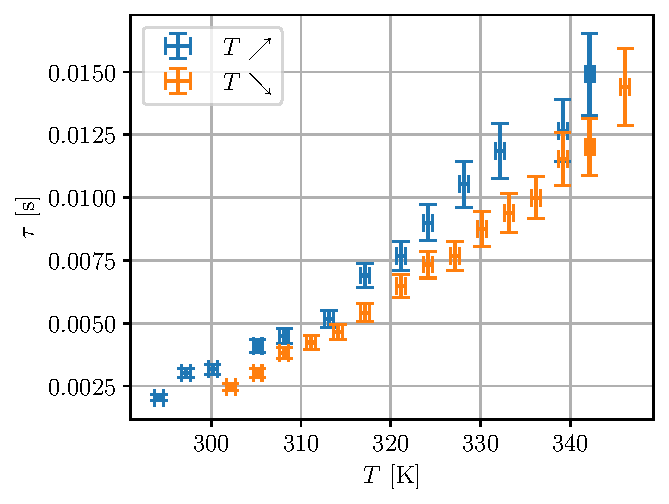
\includegraphics[width=\linewidth]{figures/huile2_tau.pdf}
        \caption{}
        \label{fig:huile2_tau}
    \end{subfigure}
    \caption{Nombre de constante de temps $\tau$ écoulées avant le début de la mesure de la vitesse pour (a) l'huile 1 et (b) l'huile 2}
\end{figure}